% =================== Appendix 1
\chapter{Background-Subtracted Efficiency}
\section{Calculating Efficiency}
\begin{figure}[]
  \centering
 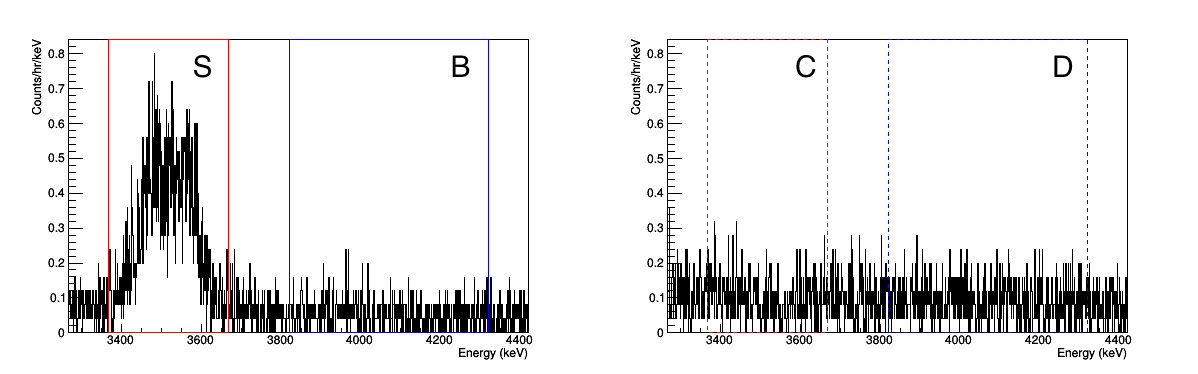
\includegraphics[width = \textwidth]{/Users/jgruszko/Documents/Thesis/Images/App1/eff_regions.png}
\caption[The energy regions used to calculate the alpha rejection efficiency]{An example of the energy regions used to calculate the alpha rejection efficiency. The spectrum with the alpha source incident on the detector surface {\it (left)} is used to define the location and width of the signal region $S$ and the location of the sideband window $B$. The same energy regions in the background spectrum {\it (right)}, $C$ and $D$, are used to determine the underlying background spectrum shape.}
\label{fig:regions}
\end{figure}

The alpha rejection efficiency of the DCR cut is evaluated using information from both a sideband and a source-free data set to estimate the background in the signal peak region. This method allows for both a non-flat background spectrum and for a varying background level over the course of the measurements. Both of these corrections are used to account for the presence of muon background events in the alpha peak regions. 
 
The energy regions used in the calculation are depicted in Fig.~\ref{fig:regions}. The signal region $S$, determined using the Gaussian fit to the alpha energy peak, is taken to be a 5$\sigma$ window centered at the peak centroid. The background sideband region $B$ is taken to be a 500\,keV window starting 5$\sigma$ above the centroid of the alpha peak. Only a right-hand-side sideband window is used, since outlier alpha events (see Sec.~\ref{sssec:outliers}) contribute to the left-hand sideband. The background spectrum energy windows $C$ and $D$ have identical energy ranges as $S$ and $B$, respectively. In each window, the event count with and without the DCR cut applied is measured. 

Of these eight measurements, only six are used to calculate the efficiency, since the DCR acceptance rate of background events is assumed to be the same in regions $B$ and $D$. Using the labels for the regions, and indicating counts without the DCR cut applied with the subscript $u$ and those with the cut applied with the subscript $s$, the DCR alpha acceptance rate is given by:
\begin{equation}
\epsilon_A = \frac{S_c - \frac{B_u C_c}{D_u}}{S_u - \frac{B_u C_u}{D_u}} = f(S_c, C_c, S_u, C_u, B_u, D_u) 
\label{eqn:eff}
\end{equation}
where the $A$ indicates the ``true," background-subtracted, alpha events. The measurements in different regions are independent of one another, and given the low statistics, they are assumed to be Poisson-distributed.

\section{Uncertainty of Efficiency}
The uncertainty of a generic non-linear function is found by Taylor expanding it to first order:
$$
f(x_1, x_2, ..., x_n) \approx f^0 + \sum_i^n \frac{\partial f}{\partial x_i} x_i
$$
where the sum is over all independent variables, and $\frac{\partial f}{\partial x_i}$ is the partial derivative of $f$, evaluated at the mean value of all measured $x_i$. Since $f^0$ is constant, it does not contribute to the uncertainty, and the variance is:
\begin{equation}
\sigma_f^2 = \sum_i^n \frac{\partial f}{\partial x_i}^2 \sigma_i^2 + \sum_i^n \sum_{j(j\ne i)}^n \frac{\partial f}{\partial x_i}\frac{\partial f}{\partial x_j} Cov.(x_i, x_j)
\label{eqn:form}
\end{equation}
This derivation assumes that the uncertainties of the measurements $\sigma_i$ are small compared to the partial derivatives, a safe assumption in this case. The numbers of counts in each measurement window are Poisson-distributed variables, so $ \sigma_{i} = \sqrt x_i $.

The covariance between measurements in difference regions is 0, since these measurements are independent. The covariance between $S_u$ and $S_c$, or between $C_u$ and $C_c$, on the other hand, is non-zero and must be calculated.

The counts in a given region with and without the DCR cut applied are binomial-distributed. Therefore, in region $S$, for example, where $\epsilon = \frac{S_c}{S_u}$, 
$$
\sigma_{\epsilon}^2 = \frac{\epsilon (1-\epsilon)}{N} = \frac{S_c (S_u - S_c)}{S_u^3} .
$$
Again using the linearized propagation of uncertainty formula, 
$$
\sigma_{\epsilon}^2 = \frac{\partial \epsilon}{\partial S_c}^2 \sigma_{S_c}^2 + \frac{\partial \epsilon}{\partial S_u}^2 \sigma_{S_u}^2 + 2 \frac{\partial \epsilon}{\partial S_c} \frac{\partial \epsilon}{\partial S_u} Cov.(S_c, S_u) 
$$
and substituting the appropriate expressions
$$
\frac{S_c (S_u - S_c)}{S_u^3} = \frac{S_c}{S_u^2} + \frac{S_c^2}{S_u^3} - 2\frac{S_c}{S_u^3} Cov.(S_c, S_u) 
$$
allows us to solve for the covariance:
$$
Cov.(S_c, S_u)  = S_c
$$
The same holds in region $C$. 

Substituting Eqn.~\ref{eqn:eff} in Eqn.~\ref{eqn:form} and writing only non-zero terms,
\begin{equation}
\openup 1\jot
\begin{split}
\sigma_{\epsilon}^2 =  &\frac{\partial \epsilon}{\partial S_c}^2 \sigma_{S_c}^2 + \frac{\partial \epsilon}{\partial S_u}^2 \sigma_{S_u}^2 + 2 \frac{\partial \epsilon}{\partial S_c} \frac{\partial \epsilon}{\partial S_u} Cov.(S_c, S_u) \\
                                       + &\frac{\partial \epsilon}{\partial C_c}^2 \sigma_{C_c}^2 + \frac{\partial \epsilon}{\partial C_u}^2 \sigma_{C_u}^2 + 2 \frac{\partial \epsilon}{\partial C_c} \frac{\partial \epsilon}{\partial C_u} Cov.(C_c, C_u) \\
                                       + &\frac{\partial \epsilon}{\partial B_u}^2 \sigma_{B_u}^2 + \frac{\partial \epsilon}{\partial D_u}^2 \sigma_{D_u}^2
\end{split}
\end{equation}
where $\epsilon = \epsilon_A$. Substituting the partial derivatives, Poisson uncertainties, and expressions for the covariances found above, results, after some manipulation, in the expression:
\begin{equation}
\openup 1\jot
\begin{split}
\sigma_{\epsilon}^2  = \frac{1}{A_u^2} \bigg[ & \left( S_c + \frac{B_u}{D_u}^2 C_c \right) \left(1 -2 \epsilon \right) \\
                                                                     & + \left( S_u + \frac{B_u}{D_u}^2 C_u \right) \epsilon^2  \\
                                                                     & + \frac{B_u}{D_u^2} \left( 1+ \frac{B_u}{D_u} \right) \left (\epsilon C_u - C_c \right)^2 \bigg]
\end{split}
\end{equation}
where $A_u = S_u - \frac{B_u C_u}{D_u}$ and $\epsilon = \epsilon_A$ is as given in Eqn.~\ref{eqn:eff}.                                                                     